3. \begin{figure}[ht!]
\center{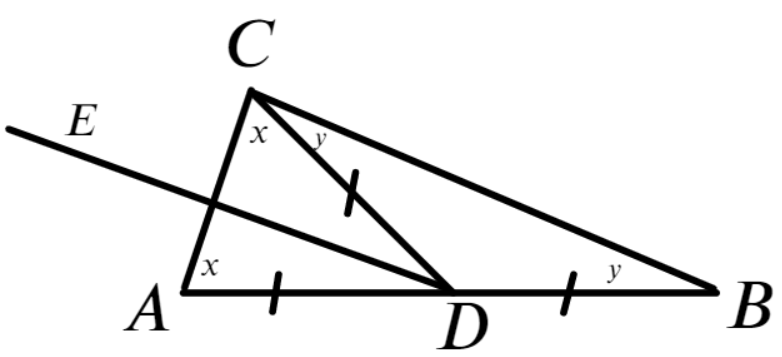
\includegraphics[scale=0.35]{g3.png}}
\end{figure}\\
Треугольники $ADC$ и $BDC$ являются равнобедренными, значит в них углы при основании равны. Обозначим $\angle CAD=\angle ACD=x,\ \angle DBC=\angle BDC=y.$ Тогда выразим сумму углов треугольника $ABC:\ 2x+2y=180^\circ,\ x+y=90^\circ\Rightarrow BC \perp AC\Rightarrow DE\perp AC,$ ч.т.д. (т.к. $DE\parallel BC$)\\
